% Options for packages loaded elsewhere
\PassOptionsToPackage{unicode}{hyperref}
\PassOptionsToPackage{hyphens}{url}
\PassOptionsToPackage{dvipsnames,svgnames,x11names}{xcolor}
%
\documentclass[
  letterpaper,
  DIV=11,
  numbers=noendperiod]{scrreprt}

\usepackage{amsmath,amssymb}
\usepackage{iftex}
\ifPDFTeX
  \usepackage[T1]{fontenc}
  \usepackage[utf8]{inputenc}
  \usepackage{textcomp} % provide euro and other symbols
\else % if luatex or xetex
  \usepackage{unicode-math}
  \defaultfontfeatures{Scale=MatchLowercase}
  \defaultfontfeatures[\rmfamily]{Ligatures=TeX,Scale=1}
\fi
\usepackage{lmodern}
\ifPDFTeX\else  
    % xetex/luatex font selection
\fi
% Use upquote if available, for straight quotes in verbatim environments
\IfFileExists{upquote.sty}{\usepackage{upquote}}{}
\IfFileExists{microtype.sty}{% use microtype if available
  \usepackage[]{microtype}
  \UseMicrotypeSet[protrusion]{basicmath} % disable protrusion for tt fonts
}{}
\makeatletter
\@ifundefined{KOMAClassName}{% if non-KOMA class
  \IfFileExists{parskip.sty}{%
    \usepackage{parskip}
  }{% else
    \setlength{\parindent}{0pt}
    \setlength{\parskip}{6pt plus 2pt minus 1pt}}
}{% if KOMA class
  \KOMAoptions{parskip=half}}
\makeatother
\usepackage{xcolor}
\setlength{\emergencystretch}{3em} % prevent overfull lines
\setcounter{secnumdepth}{5}
% Make \paragraph and \subparagraph free-standing
\makeatletter
\ifx\paragraph\undefined\else
  \let\oldparagraph\paragraph
  \renewcommand{\paragraph}{
    \@ifstar
      \xxxParagraphStar
      \xxxParagraphNoStar
  }
  \newcommand{\xxxParagraphStar}[1]{\oldparagraph*{#1}\mbox{}}
  \newcommand{\xxxParagraphNoStar}[1]{\oldparagraph{#1}\mbox{}}
\fi
\ifx\subparagraph\undefined\else
  \let\oldsubparagraph\subparagraph
  \renewcommand{\subparagraph}{
    \@ifstar
      \xxxSubParagraphStar
      \xxxSubParagraphNoStar
  }
  \newcommand{\xxxSubParagraphStar}[1]{\oldsubparagraph*{#1}\mbox{}}
  \newcommand{\xxxSubParagraphNoStar}[1]{\oldsubparagraph{#1}\mbox{}}
\fi
\makeatother

\usepackage{color}
\usepackage{fancyvrb}
\newcommand{\VerbBar}{|}
\newcommand{\VERB}{\Verb[commandchars=\\\{\}]}
\DefineVerbatimEnvironment{Highlighting}{Verbatim}{commandchars=\\\{\}}
% Add ',fontsize=\small' for more characters per line
\usepackage{framed}
\definecolor{shadecolor}{RGB}{241,243,245}
\newenvironment{Shaded}{\begin{snugshade}}{\end{snugshade}}
\newcommand{\AlertTok}[1]{\textcolor[rgb]{0.68,0.00,0.00}{#1}}
\newcommand{\AnnotationTok}[1]{\textcolor[rgb]{0.37,0.37,0.37}{#1}}
\newcommand{\AttributeTok}[1]{\textcolor[rgb]{0.40,0.45,0.13}{#1}}
\newcommand{\BaseNTok}[1]{\textcolor[rgb]{0.68,0.00,0.00}{#1}}
\newcommand{\BuiltInTok}[1]{\textcolor[rgb]{0.00,0.23,0.31}{#1}}
\newcommand{\CharTok}[1]{\textcolor[rgb]{0.13,0.47,0.30}{#1}}
\newcommand{\CommentTok}[1]{\textcolor[rgb]{0.37,0.37,0.37}{#1}}
\newcommand{\CommentVarTok}[1]{\textcolor[rgb]{0.37,0.37,0.37}{\textit{#1}}}
\newcommand{\ConstantTok}[1]{\textcolor[rgb]{0.56,0.35,0.01}{#1}}
\newcommand{\ControlFlowTok}[1]{\textcolor[rgb]{0.00,0.23,0.31}{\textbf{#1}}}
\newcommand{\DataTypeTok}[1]{\textcolor[rgb]{0.68,0.00,0.00}{#1}}
\newcommand{\DecValTok}[1]{\textcolor[rgb]{0.68,0.00,0.00}{#1}}
\newcommand{\DocumentationTok}[1]{\textcolor[rgb]{0.37,0.37,0.37}{\textit{#1}}}
\newcommand{\ErrorTok}[1]{\textcolor[rgb]{0.68,0.00,0.00}{#1}}
\newcommand{\ExtensionTok}[1]{\textcolor[rgb]{0.00,0.23,0.31}{#1}}
\newcommand{\FloatTok}[1]{\textcolor[rgb]{0.68,0.00,0.00}{#1}}
\newcommand{\FunctionTok}[1]{\textcolor[rgb]{0.28,0.35,0.67}{#1}}
\newcommand{\ImportTok}[1]{\textcolor[rgb]{0.00,0.46,0.62}{#1}}
\newcommand{\InformationTok}[1]{\textcolor[rgb]{0.37,0.37,0.37}{#1}}
\newcommand{\KeywordTok}[1]{\textcolor[rgb]{0.00,0.23,0.31}{\textbf{#1}}}
\newcommand{\NormalTok}[1]{\textcolor[rgb]{0.00,0.23,0.31}{#1}}
\newcommand{\OperatorTok}[1]{\textcolor[rgb]{0.37,0.37,0.37}{#1}}
\newcommand{\OtherTok}[1]{\textcolor[rgb]{0.00,0.23,0.31}{#1}}
\newcommand{\PreprocessorTok}[1]{\textcolor[rgb]{0.68,0.00,0.00}{#1}}
\newcommand{\RegionMarkerTok}[1]{\textcolor[rgb]{0.00,0.23,0.31}{#1}}
\newcommand{\SpecialCharTok}[1]{\textcolor[rgb]{0.37,0.37,0.37}{#1}}
\newcommand{\SpecialStringTok}[1]{\textcolor[rgb]{0.13,0.47,0.30}{#1}}
\newcommand{\StringTok}[1]{\textcolor[rgb]{0.13,0.47,0.30}{#1}}
\newcommand{\VariableTok}[1]{\textcolor[rgb]{0.07,0.07,0.07}{#1}}
\newcommand{\VerbatimStringTok}[1]{\textcolor[rgb]{0.13,0.47,0.30}{#1}}
\newcommand{\WarningTok}[1]{\textcolor[rgb]{0.37,0.37,0.37}{\textit{#1}}}

\providecommand{\tightlist}{%
  \setlength{\itemsep}{0pt}\setlength{\parskip}{0pt}}\usepackage{longtable,booktabs,array}
\usepackage{calc} % for calculating minipage widths
% Correct order of tables after \paragraph or \subparagraph
\usepackage{etoolbox}
\makeatletter
\patchcmd\longtable{\par}{\if@noskipsec\mbox{}\fi\par}{}{}
\makeatother
% Allow footnotes in longtable head/foot
\IfFileExists{footnotehyper.sty}{\usepackage{footnotehyper}}{\usepackage{footnote}}
\makesavenoteenv{longtable}
\usepackage{graphicx}
\makeatletter
\newsavebox\pandoc@box
\newcommand*\pandocbounded[1]{% scales image to fit in text height/width
  \sbox\pandoc@box{#1}%
  \Gscale@div\@tempa{\textheight}{\dimexpr\ht\pandoc@box+\dp\pandoc@box\relax}%
  \Gscale@div\@tempb{\linewidth}{\wd\pandoc@box}%
  \ifdim\@tempb\p@<\@tempa\p@\let\@tempa\@tempb\fi% select the smaller of both
  \ifdim\@tempa\p@<\p@\scalebox{\@tempa}{\usebox\pandoc@box}%
  \else\usebox{\pandoc@box}%
  \fi%
}
% Set default figure placement to htbp
\def\fps@figure{htbp}
\makeatother
% definitions for citeproc citations
\NewDocumentCommand\citeproctext{}{}
\NewDocumentCommand\citeproc{mm}{%
  \begingroup\def\citeproctext{#2}\cite{#1}\endgroup}
\makeatletter
 % allow citations to break across lines
 \let\@cite@ofmt\@firstofone
 % avoid brackets around text for \cite:
 \def\@biblabel#1{}
 \def\@cite#1#2{{#1\if@tempswa , #2\fi}}
\makeatother
\newlength{\cslhangindent}
\setlength{\cslhangindent}{1.5em}
\newlength{\csllabelwidth}
\setlength{\csllabelwidth}{3em}
\newenvironment{CSLReferences}[2] % #1 hanging-indent, #2 entry-spacing
 {\begin{list}{}{%
  \setlength{\itemindent}{0pt}
  \setlength{\leftmargin}{0pt}
  \setlength{\parsep}{0pt}
  % turn on hanging indent if param 1 is 1
  \ifodd #1
   \setlength{\leftmargin}{\cslhangindent}
   \setlength{\itemindent}{-1\cslhangindent}
  \fi
  % set entry spacing
  \setlength{\itemsep}{#2\baselineskip}}}
 {\end{list}}
\usepackage{calc}
\newcommand{\CSLBlock}[1]{\hfill\break\parbox[t]{\linewidth}{\strut\ignorespaces#1\strut}}
\newcommand{\CSLLeftMargin}[1]{\parbox[t]{\csllabelwidth}{\strut#1\strut}}
\newcommand{\CSLRightInline}[1]{\parbox[t]{\linewidth - \csllabelwidth}{\strut#1\strut}}
\newcommand{\CSLIndent}[1]{\hspace{\cslhangindent}#1}

\usepackage{booktabs}
\usepackage{caption}
\usepackage{longtable}
\usepackage{colortbl}
\usepackage{array}
\usepackage{anyfontsize}
\usepackage{multirow}
\KOMAoption{captions}{tableheading}
\makeatletter
\@ifpackageloaded{bookmark}{}{\usepackage{bookmark}}
\makeatother
\makeatletter
\@ifpackageloaded{caption}{}{\usepackage{caption}}
\AtBeginDocument{%
\ifdefined\contentsname
  \renewcommand*\contentsname{Table of contents}
\else
  \newcommand\contentsname{Table of contents}
\fi
\ifdefined\listfigurename
  \renewcommand*\listfigurename{List of Figures}
\else
  \newcommand\listfigurename{List of Figures}
\fi
\ifdefined\listtablename
  \renewcommand*\listtablename{List of Tables}
\else
  \newcommand\listtablename{List of Tables}
\fi
\ifdefined\figurename
  \renewcommand*\figurename{Figure}
\else
  \newcommand\figurename{Figure}
\fi
\ifdefined\tablename
  \renewcommand*\tablename{Table}
\else
  \newcommand\tablename{Table}
\fi
}
\@ifpackageloaded{float}{}{\usepackage{float}}
\floatstyle{ruled}
\@ifundefined{c@chapter}{\newfloat{codelisting}{h}{lop}}{\newfloat{codelisting}{h}{lop}[chapter]}
\floatname{codelisting}{Listing}
\newcommand*\listoflistings{\listof{codelisting}{List of Listings}}
\makeatother
\makeatletter
\makeatother
\makeatletter
\@ifpackageloaded{caption}{}{\usepackage{caption}}
\@ifpackageloaded{subcaption}{}{\usepackage{subcaption}}
\makeatother

\usepackage{bookmark}

\IfFileExists{xurl.sty}{\usepackage{xurl}}{} % add URL line breaks if available
\urlstyle{same} % disable monospaced font for URLs
\hypersetup{
  pdftitle={physics-manual},
  pdfauthor={Physics - Tallaght},
  colorlinks=true,
  linkcolor={blue},
  filecolor={Maroon},
  citecolor={Blue},
  urlcolor={Blue},
  pdfcreator={LaTeX via pandoc}}


\title{physics-manual}
\author{Physics - Tallaght}
\date{Invalid Date}

\begin{document}
\maketitle

\renewcommand*\contentsname{Table of contents}
{
\hypersetup{linkcolor=}
\setcounter{tocdepth}{2}
\tableofcontents
}

\bookmarksetup{startatroot}

\chapter*{Preface}\label{preface}
\addcontentsline{toc}{chapter}{Preface}

\markboth{Preface}{Preface}

This is a Quarto book.

To learn more about Quarto books visit
\url{https://quarto.org/docs/books}.

\begin{Shaded}
\begin{Highlighting}[]
\DecValTok{1} \SpecialCharTok{+} \DecValTok{1}
\end{Highlighting}
\end{Shaded}

\begin{verbatim}
[1] 2
\end{verbatim}

\bookmarksetup{startatroot}

\chapter{Simple Pendulum}\label{simple-pendulum}

Take down the following in to your laboratory copy.

\subsection{Title: Simple Pendulum}\label{title-simple-pendulum}

\subsection{Date:}\label{date}

\subsection{Partner:}\label{partner}

\subsection{Data}\label{data}

\begin{table}
\fontsize{12.0pt}{14.0pt}\selectfont
\begin{tabular*}{\linewidth}{@{\extracolsep{\fill}}>{\centering\arraybackslash}p{\dimexpr 120.00pt -2\tabcolsep-1.5\arrayrulewidth}>{\raggedleft\arraybackslash}p{\dimexpr 120.00pt -2\tabcolsep-1.5\arrayrulewidth}>{\raggedleft\arraybackslash}p{\dimexpr 120.00pt -2\tabcolsep-1.5\arrayrulewidth}>{\raggedleft\arraybackslash}p{\dimexpr 120.00pt -2\tabcolsep-1.5\arrayrulewidth}>{\raggedleft\arraybackslash}p{\dimexpr 120.00pt -2\tabcolsep-1.5\arrayrulewidth}}
\toprule
Length (m) & Actual Length (m) & \(T_{20}(s)\) & \(T_{1}(s)\) & \(T_{1}^2(s^2)\) \\ 
\midrule\addlinespace[2.5pt]
0.100 &  &  &  &  \\ 
0.200 &  &  &  &  \\ 
0.300 &  &  &  &  \\ 
0.400 &  &  &  &  \\ 
0.500 &  &  &  &  \\ 
0.600 &  &  &  &  \\ 
0.700 &  &  &  &  \\ 
0.800 &  &  &  &  \\ 
0.900 &  &  &  &  \\ 
1.000 &  &  &  &  \\ 
\bottomrule
\end{tabular*}
\end{table}

\bookmarksetup{startatroot}

\chapter{Simple Harmonic Motion of a
Spring}\label{simple-harmonic-motion-of-a-spring}

As we saw in the previous experiment, every spring has a
\emph{stiffness} called its \textbf{\emph{Spring Constant}}, \(k\),
measured in Newtons per metre. Stiff, rigid springs have high values of
\(k\), loose, floppy springs have low values of \(k\). We're going to
measure \(k\) by a totally separate mechanism and compare the new value
we get to the previous result.

Take down the following in to your laboratory copy.

\subsection{\texorpdfstring{{Title: Simple Harmonic Motion of a
Spring}}{Title: Simple Harmonic Motion of a Spring}}\label{title-simple-harmonic-motion-of-a-spring}

\subsection{\texorpdfstring{{Name:}}{Name:}}\label{name}

\subsection{\texorpdfstring{{Date:}}{Date:}}\label{date-1}

\subsection{\texorpdfstring{{Partner:}}{Partner:}}\label{partner-1}

\subsection{\texorpdfstring{{Data:}}{Data:}}\label{data-1}

\begin{table}
\fontsize{13.0pt}{15.0pt}\selectfont
\begin{tabular*}{0.85\linewidth}{@{\extracolsep{\fill}}>{\centering\arraybackslash}p{\dimexpr 90.00pt -2\tabcolsep-1.5\arrayrulewidth}>{\centering\arraybackslash}p{\dimexpr 90.00pt -2\tabcolsep-1.5\arrayrulewidth}>{\centering\arraybackslash}p{\dimexpr 90.00pt -2\tabcolsep-1.5\arrayrulewidth}>{\centering\arraybackslash}p{\dimexpr 90.00pt -2\tabcolsep-1.5\arrayrulewidth}}
\toprule
Mass (kg) & \(T_{20}(s)\) & \(T_{1}(s)\) & \(T_{1}^2(s^2)\) \\ 
\midrule\addlinespace[2.5pt]
0.300 &  &  &  \\ 
0.400 &  &  &  \\ 
0.500 &  &  &  \\ 
0.600 &  &  &  \\ 
0.700 &  &  &  \\ 
0.800 &  &  &  \\ 
0.900 &  &  &  \\ 
1.000 &  &  &  \\ 
\bottomrule
\end{tabular*}
\end{table}

\subsection{Experimental Set-Up}\label{experimental-set-up}

\pandocbounded{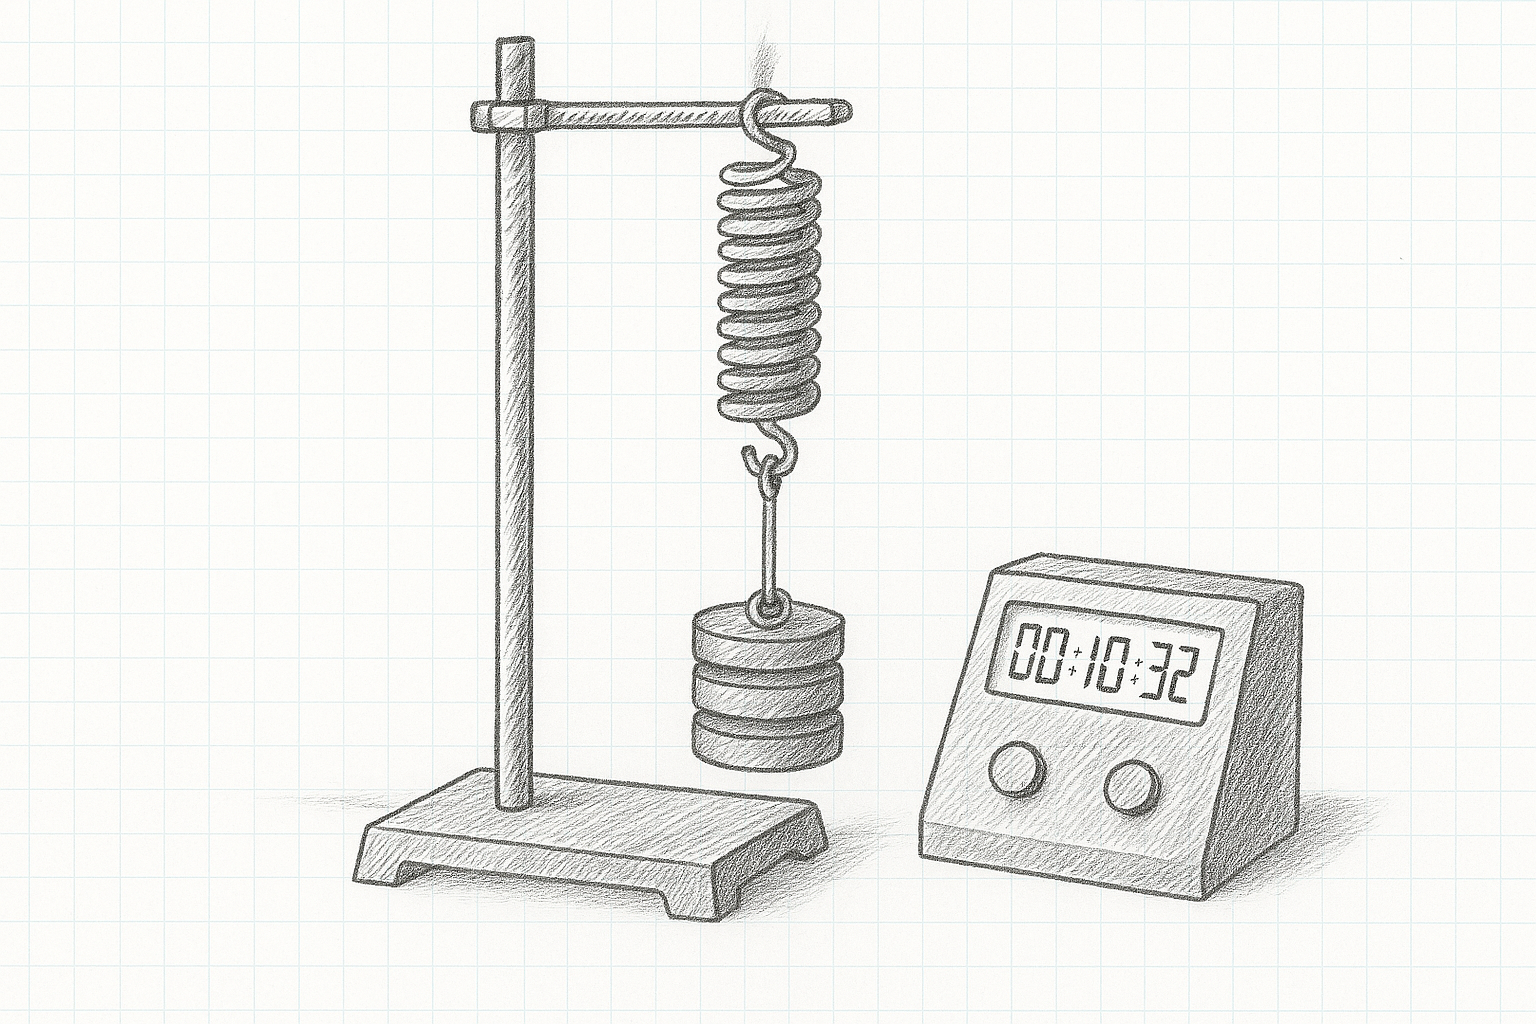
\includegraphics[keepaspectratio]{images/shm-diagram3.png}}

The apparatus will be set-up something like the sketch on the left. This
is the first point; the weight holder and two 100g weights giving a
total load of 0.300 kg.

Pull the weights down slightly and release, the weights will bounce
rapidly. With the centisecond timer, record the time for 20 bounces.
Divide this by 20 to get the time for one bounce, and then square this
value to get \(T^2\). Pay special attention to significant figures

\begin{itemize}
\item
  you get best results for small displacements, only pull the weights
  down the smallest amount you can.
\item
  One \textbf{\emph{tick}} happens every time the weights hit the bottom
  of their travel, so \emph{down, down, down} rather than \emph{up,
  down, up, down}.
\item
  0.300 kg is the weight holder and \textbf{2} extra weights
\item
  When filling out your table, pay special attention to significant
  figures. The number of significant figures for \(T_{20}\) should be
  the same as for \(T_1\) and \(T^2\).
\end{itemize}

\subsection{Analysis}\label{analysis}

\pandocbounded{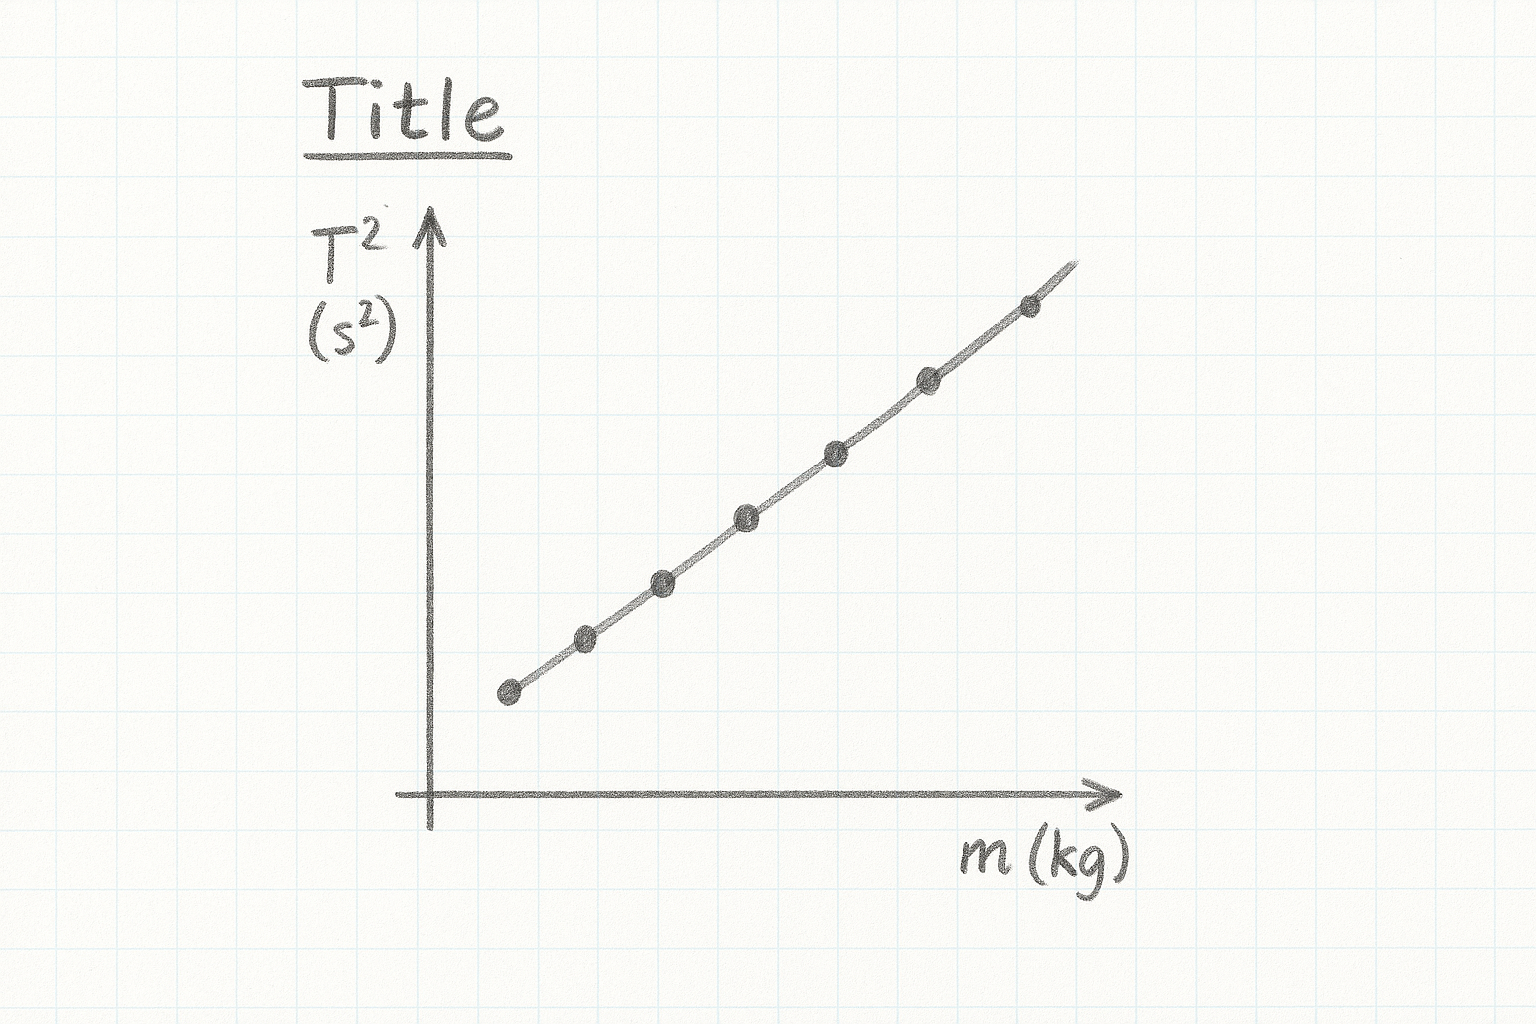
\includegraphics[keepaspectratio]{images/graph.png}}

Draw the graph as shown on the left here, with \(T^2(s^2)\) on the
y-axis and \(m(kg)\) on the x axis. Don't be surprised if there is a
reasonable amount of scatter in the points. Draw a best fit line nested
through the points. Make sure the graph has a (long) descriptive title
in the form \emph{What's on y-axis vs What's on x axis and the context}.

Calculate the slope of the best fit line using the formula
\(slope \; = \; \frac{y_2-y_1}{x_2-x_1}\)

\subsection{Calculation of the Spring Constant,
k}\label{calculation-of-the-spring-constant-k}

The equation governing the simple harmonic motion of the spring is:

\(T \; = \; 2 \pi \sqrt{\frac{k}{m}}\)

Where \(T\) is the period we measured for each mass, \(m\), and \(k\) is
the spring constant that we're setting out to measure.

Squaring and rearranging gives:

\(T^2\; = \; \frac{4\pi^2}{k} \times m\)

This means the slope of our \(T^2 \; vs \; m\) graph must be:

\(slope \; = \; \frac{4\pi^2}{k}\)

\(\implies\; k \; = \; \frac{4\pi^2}{slope}\)

Use this to calculate a value for k in N/m

\subsection{Discussion}\label{discussion}

There are four parts to the discussion section:

\begin{itemize}
\item
  \textbf{\emph{the main results}} - repeat the value of k obtained from
  the end of your calculations. Even though it is written elsewhere in
  your report, it's important to repeat it here
\item
  \textbf{\emph{the text book (manufacturers) value}} - the springs used
  have a rated k value of 100 N/m
\item
  \textbf{\emph{inaccuracies}} - your value for \(k\) won't be exactly
  the same as the manufacturers, nor will your graph be a perfect
  straight line. We need to try and account for these discrepancies.
  Pick one feature of the experiment and investigate whether it is an
  issue in the accuracy of your results. For example, are the weights
  all exactly 100g, does the amplitude of the spring oscillations
  matter, is there signs of anharmonic behaviour at heavier masses, or
  is 20 bounces enough. You'll need to examine the results you have
  already as well as gathering additional evidence by taking further
  measurements. Your idea might well be a key issue in the quality of
  the results we obtain, or it might not be and you are thus ruling it
  out. Both are valid outcomes of this error analysis.
\item
  \textbf{\emph{improvements}} - based on the inaccuracy section above,
  can you suggest a way in which we could make our experiment better?
\end{itemize}

\subsection{Apparatus}\label{apparatus}

Retort stand, weight holder, 9 \(\times\) 100g weights, centisecond
timer, 100 N/m spring.

\bookmarksetup{startatroot}

\chapter{Measurement of Acceleration on a Linear
Air-Track}\label{measurement-of-acceleration-on-a-linear-air-track}

Today we're going to investigate the kinematic equations of motion,
specifically \(s \; = \; v_0 t \; + \; \frac{1}{2} a t^2\). To do this
we need constant acceleration in a frictionless environment and to
achieve this we use an \emph{air track} where a glider floats on a
cushion of air blown through holes in the track.

Take down the following in to your laboratory copy.

\subsection{\texorpdfstring{{Measurement of Acceleration on a Linear Air
Track}}{Measurement of Acceleration on a Linear Air Track}}\label{measurement-of-acceleration-on-a-linear-air-track-1}

\subsection{\texorpdfstring{{Name:}}{Name:}}\label{name-1}

\subsection{\texorpdfstring{{Date:}}{Date:}}\label{date-2}

\subsection{\texorpdfstring{{Partner:}}{Partner:}}\label{partner-2}

\subsection{\texorpdfstring{{Data:}}{Data:}}\label{data-2}

\begin{table}
\fontsize{13.0pt}{15.0pt}\selectfont
\begin{tabular*}{0.85\linewidth}{@{\extracolsep{\fill}}>{\centering\arraybackslash}p{\dimexpr 90.00pt -2\tabcolsep-1.5\arrayrulewidth}>{\centering\arraybackslash}p{\dimexpr 90.00pt -2\tabcolsep-1.5\arrayrulewidth}>{\centering\arraybackslash}p{\dimexpr 90.00pt -2\tabcolsep-1.5\arrayrulewidth}}
\toprule
s(m) & \(t(s)\) & \(t^2(s^2)\) \\ 
\midrule\addlinespace[2.5pt]
0.200 &  &  \\ 
0.300 &  &  \\ 
0.400 &  &  \\ 
0.500 &  &  \\ 
0.600 &  &  \\ 
0.700 &  &  \\ 
0.800 &  &  \\ 
\bottomrule
\end{tabular*}
\end{table}

\subsection{Experimental Set-Up}\label{experimental-set-up-1}

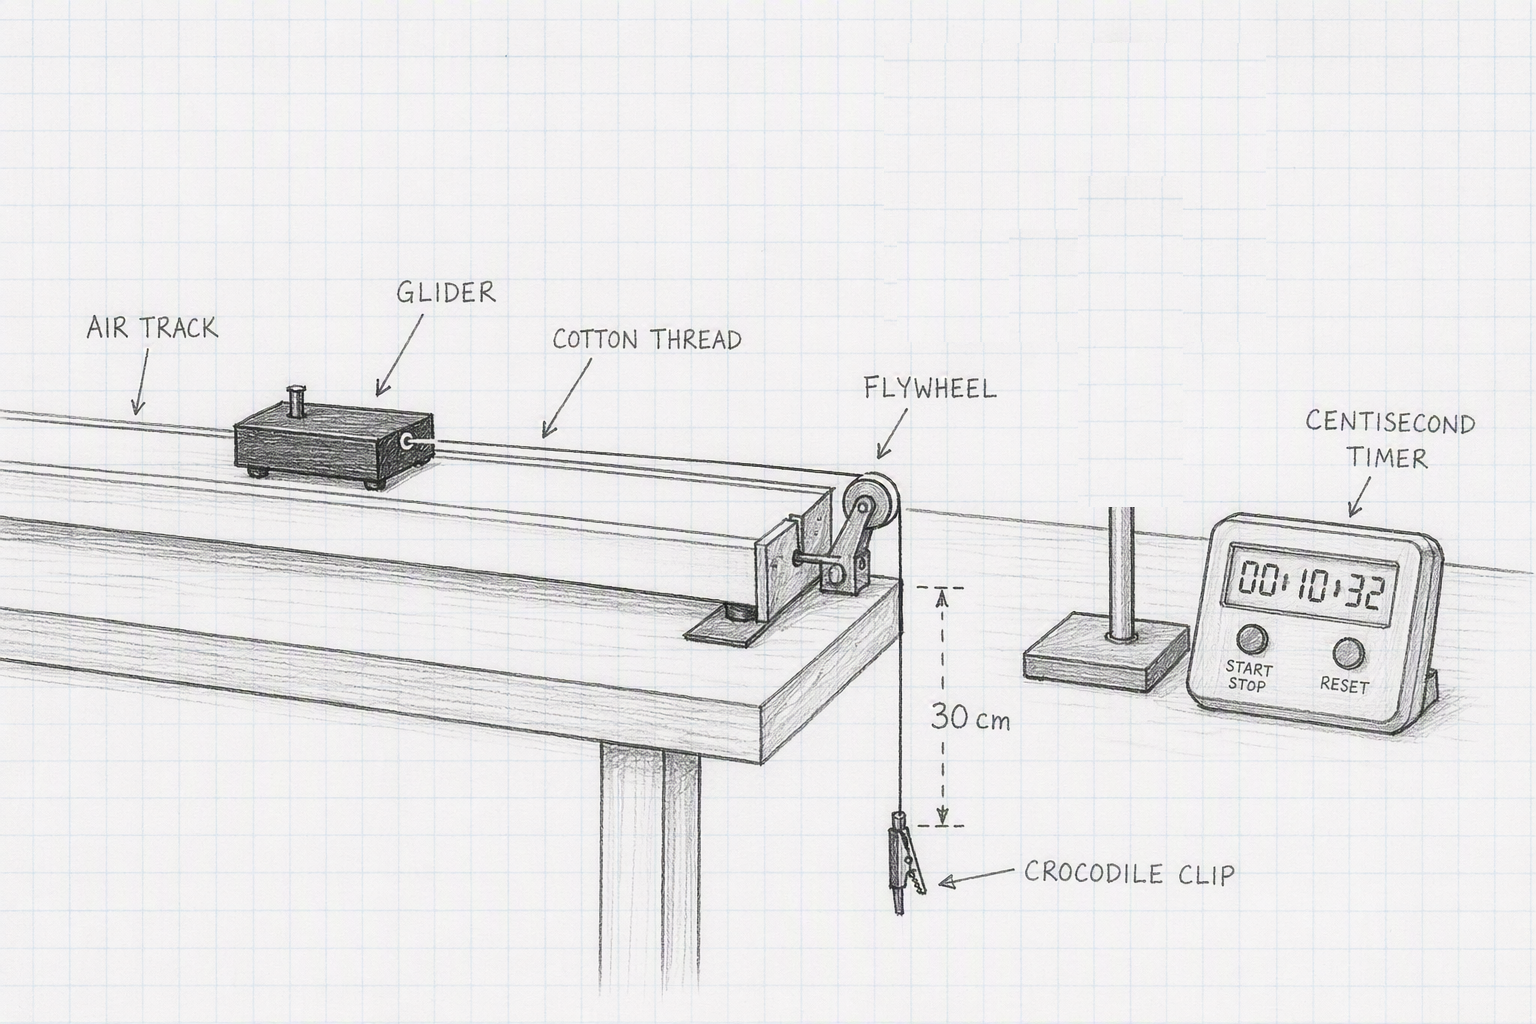
\includegraphics[width=10cm,height=5cm]{images/air-track.png}

The apparatus will be set-up something like the sketch on the left. The
glider is pulled back so that its front edge just touches the 0.300m
point on the track. It is gently released and will accelerate towards
the end of the track. The timer is started whhen the glider is released,
and is stopped as the front edge of the glider passes the 0.100m mark on
the track. This is the first point, s = 0.200m

\begin{itemize}
\item
  before you begin your measurements make sure the track is level by
  detaching the cotton thread from the glider and seeing if the glider
  moves off in any direction. If not level, the track can be adjusted by
  the rubber screws on each leg.
\item
  make sure you release the glider from rest, without giving it a push
  in either direction
\item
  make sure the crocodile clip is still above ground when the glider
  passes the finish (0.100m) line so that it is always accelerating.
\item
  check to make sure the cotton thread is still running over the
  flywheel after each measurement.
\item
  When filling out your table, pay special attention to significant
  figures. The number of significant figures for \(t\) should be the
  same as for \(t^2\).
\end{itemize}

\subsection{Analysis}\label{analysis-1}

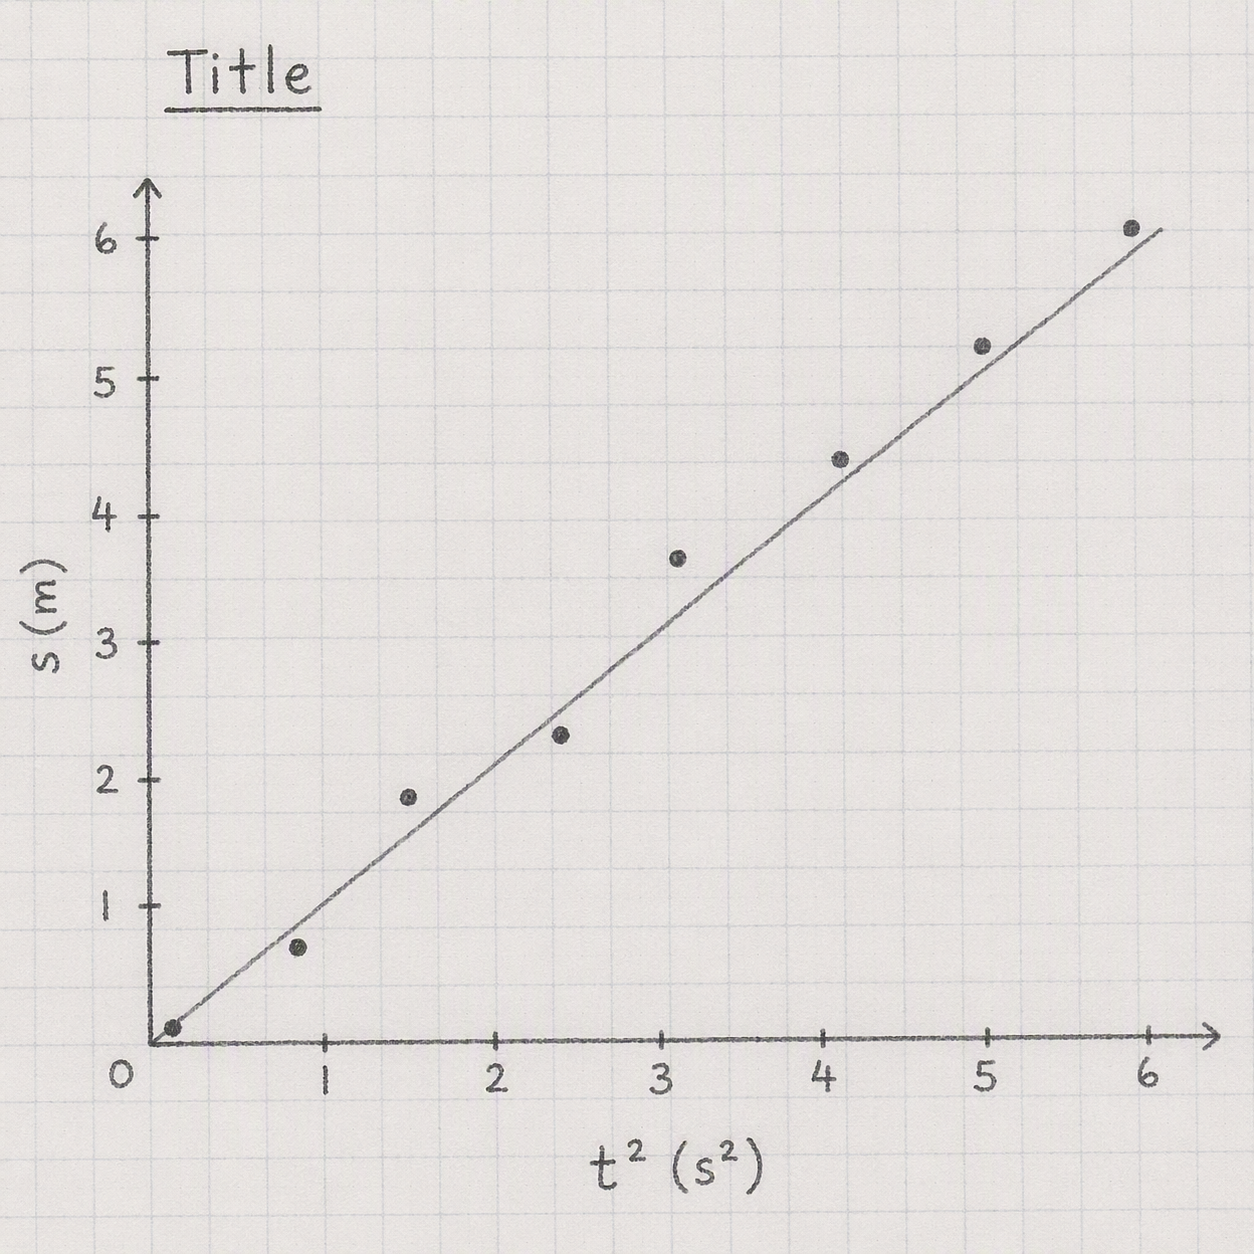
\includegraphics[width=10cm,height=6cm]{images/air-track-graph.png}

Draw the graph as shown on the left here, with \(t^2(s^2)\) on the
x-axis and \(s(m)\) on the y axis. Don't be surprised if there is a
reasonable amount of scatter in the points. Draw a best fit line nested
through the points. Make sure the graph has a (long) descriptive title
in the form \emph{What's on y-axis vs What's on x axis and the context}.

Calculate the slope of the best fit line using the formula
\(slope \; = \; \frac{y_2-y_1}{x_2-x_1}\)

\subsection{Calculation of the acceleration,
a}\label{calculation-of-the-acceleration-a}

The kinematic equation of relevance here is:

\(s \; = \; v_0 t \; + \; \frac{1}{2} a t^2\)

Where \(v_o\) is the initial velocity which will be zero and we can
ignore that. So \(s \; = \; \frac{1}{2} a t^2\).

This means the slope of our graph will be \(\frac{1}{2}a\) so \(a\) is
twice the slope.

We're going to check on our acceleration value by a separate set of
measurements. Detach the crocodile clip and the glider from the
apparatus and weight each separately, let's call the results
\(m_{glider}\) and \(m_{clip}\). From Newton's Laws, \(F \; = \; ma\)
where in this ccase the force causing the acceleration is the weight of
the clip, \(F = W = m_{clip} \times g\) and \(m\) is the
\(total \; mass = m_{glider} + m_{clip}\).

So we get
\(a_{theory} = \frac{m_{clip} \times g}{m_{glider} + m_{clip}}\). Use
the masses you measured and \(g = 9.81 \; m/s^2\) to work out this
second value for \(a\).

\subsection{Discussion}\label{discussion-1}

There are four parts to the discussion section:

\begin{itemize}
\item
  \textbf{\emph{the main results}} - repeat the value of \emph{\(a\)}
  obtained from the end of your calculations. Even though it is written
  elsewhere in your report, it's important to repeat it here.
\item
  \textbf{\emph{the text book (reference) value}} - repeat the value you
  have for \(a_{theory}\) here.
\item
  \textbf{\emph{inaccuracies}} - your values for \(a\) won't be exactly
  the same, nor will your graph be a perfect straight line. We need to
  try and account for these discrepancies. Pick one feature of the
  experiment and investigate whether it is an issue in the accuracy of
  your results. For example, how reliable are the (very short) times
  measured in the results table, maybe we should repeat for one value of
  \(s\) and see how consistent they are. You'll need to examine the
  results you have already as well as gathering additional evidence by
  taking further measurements. Your idea might well be a key issue in
  the quality of the results we obtain, or it might not be and you are
  thus ruling it out. Both are valid outcomes of this error analysis.
\item
  \textbf{\emph{improvements}} - based on the inaccuracy section above,
  can you suggest a way in which we could make our experiment better?
\end{itemize}

\subsection{Apparatus}\label{apparatus-1}

Levelled linear air track with glider in place attached to a cotton
thread which runs frictionlessly over a flywheel. The thread is long
enough to hit the floor with the glider at the end of its travel.. A
centisecond timer. Weighing scales with a range of at least 0-200g and a
sensitivity of 0.01g.

\bookmarksetup{startatroot}

\chapter{Coefficient of Restitution of a Ping Pong
Ball}\label{coefficient-of-restitution-of-a-ping-pong-ball}

In any collision there is balance between elastic and inelastic forces.
Inelastic forces lead to losses in mechanical energies and dissipation
of such energies in the form of non-mechanical energies such as heat and
sound. The parameter that describes how elastic a collision is is called
the Coefficient of Restitution (COR). It is a dimensionless number that
essentially says how bouncy something is; for a rubber super ball it'll
be close to 1, for a water balloon it'll be close to zero. We're going
to measure this for a ping pong ball by dropping it from various heights
and recording how high it rebounds.

Take down the following in to your laboratory copy.

\subsection{\texorpdfstring{{Title: Coefficient of Restitution of a Ping
Pong
Ball}}{Title: Coefficient of Restitution of a Ping Pong Ball}}\label{title-coefficient-of-restitution-of-a-ping-pong-ball}

\subsection{\texorpdfstring{{Name:}}{Name:}}\label{name-2}

\subsection{\texorpdfstring{{Date:}}{Date:}}\label{date-3}

\subsection{\texorpdfstring{{Partner:}}{Partner:}}\label{partner-3}

\subsection{\texorpdfstring{{Data:}}{Data:}}\label{data-3}

\begin{table}
\fontsize{13.0pt}{15.0pt}\selectfont
\begin{tabular*}{0.85\linewidth}{@{\extracolsep{\fill}}>{\centering\arraybackslash}p{\dimexpr 75.00pt -2\tabcolsep-1.5\arrayrulewidth}>{\centering\arraybackslash}p{\dimexpr 60.00pt -2\tabcolsep-1.5\arrayrulewidth}>{\centering\arraybackslash}p{\dimexpr 45.00pt -2\tabcolsep-1.5\arrayrulewidth}>{\centering\arraybackslash}p{\dimexpr 45.00pt -2\tabcolsep-1.5\arrayrulewidth}>{\centering\arraybackslash}p{\dimexpr 45.00pt -2\tabcolsep-1.5\arrayrulewidth}>{\centering\arraybackslash}p{\dimexpr 45.00pt -2\tabcolsep-1.5\arrayrulewidth}>{\centering\arraybackslash}p{\dimexpr 45.00pt -2\tabcolsep-1.5\arrayrulewidth}>{\centering\arraybackslash}p{\dimexpr 45.00pt -2\tabcolsep-1.5\arrayrulewidth}>{\centering\arraybackslash}p{\dimexpr 45.00pt -2\tabcolsep-1.5\arrayrulewidth}}
\toprule
Drop(m) & \(B_1(m)\) & \(B_2(m)\) & \(B_3(m)\) & \(B_4(m)\) & \(B_5(m)\) & \(B_{av}(m)\) & \(B_{min}(m)\) & \(B_{max}(m)\) \\ 
\midrule\addlinespace[2.5pt]
0.600 &  &  &  &  &  &  &  &  \\ 
0.800 &  &  &  &  &  &  &  &  \\ 
1.000 &  &  &  &  &  &  &  &  \\ 
1.200 &  &  &  &  &  &  &  &  \\ 
1.400 &  &  &  &  &  &  &  &  \\ 
1.600 &  &  &  &  &  &  &  &  \\ 
1.800 &  &  &  &  &  &  &  &  \\ 
2.000 &  &  &  &  &  &  &  &  \\ 
\bottomrule
\end{tabular*}
\end{table}

\subsection{Experimental Set-Up}\label{experimental-set-up-2}

The table tennis ball is dropped from various height in front of the
metre sticks and the bounce height recorded. Because it is difficult to
accurately record the bounce height, each measurement is repeated five
times and an average is taken. The \(B_{av}\) column is the averagee for
the five bounces for a particular drop height, making sure you have the
right number of significant figures in \(B_{av}\). The \(B_{min}\) and
\(B_{max}\) columns are the smallest and largets of the five
measurements

Things to watch out for:

\begin{itemize}
\item
  because floor level is at 0.000m, measure the drop height and the
  bounce heights from the \textbf{\emph{bottom}} of the ping pong ball.
\item
  because things happen fast, it can be useful to video record the
  bounce on your phone to capture the apex of the bounce.
\end{itemize}

\newpage{}

\subsection{Analysis}\label{analysis-2}

\pandocbounded{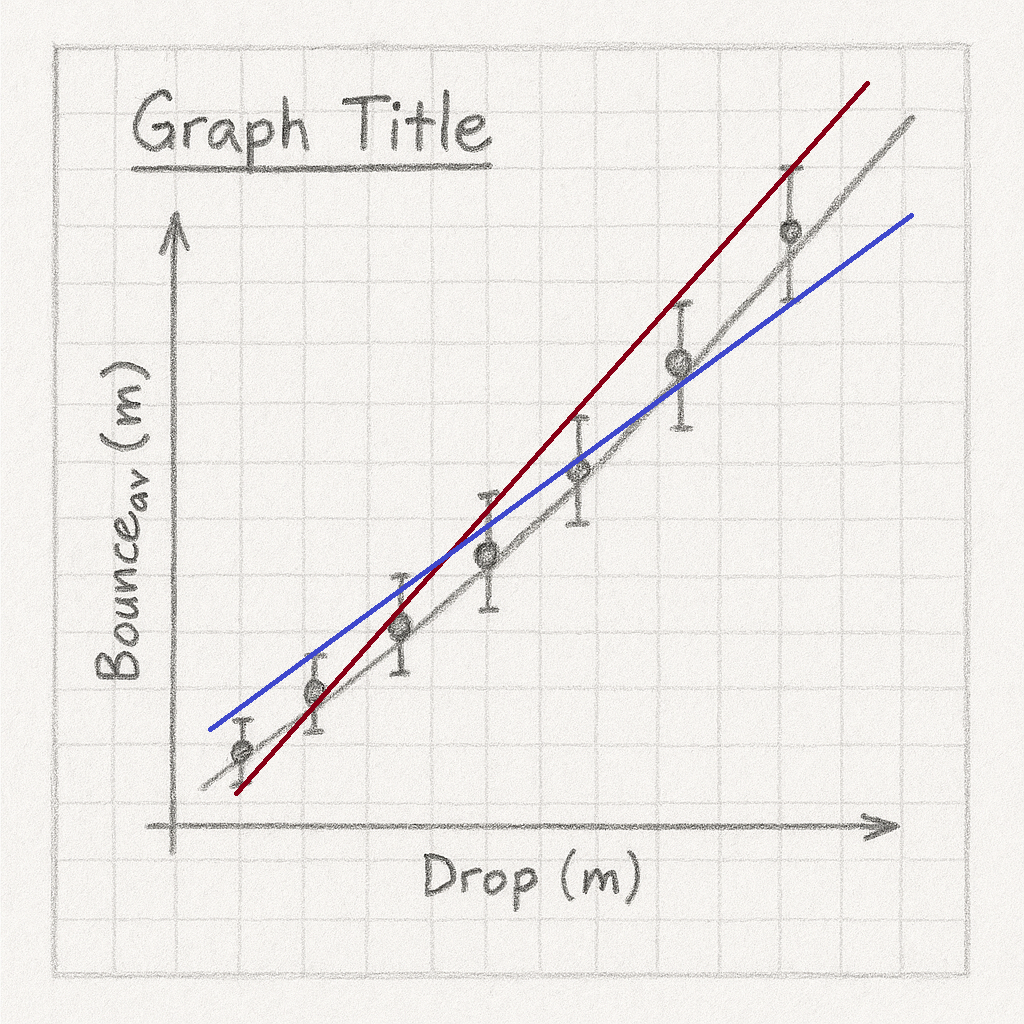
\includegraphics[keepaspectratio]{images/cor-graph-3-lines.png}}

Draw the graph as shown on the left here, with \(B_{av}(m)\) on the
y-axis and \(Drop(m)\) on the x axis. Don't be surprised if there is a
reasonable amount of scatter in the points. Instead of drawing circles
around each point, we'll represent them by chi-fighter like points where
the centre dot is at \(B_{av}\), the top line at \(B_{max}\), and the
bottom line at \(B_{min}\). Draw a best fit line nested through the
points. Draw a steepest possible line \textasciitilde consistent with
the chi-fighters (shown in red pencil in our graph here). Draw a
shallowest possible line \textasciitilde consistent with the
chi-fighters (shown in blue). Calculate the slopes of all three lines

\subsection{Calculation of the COR}\label{calculation-of-the-cor}

The equation governing COR is:

\(COR \; = \; \frac{speed\ of\ separation\ after\ impct}{speed\ of\ approach\ before\ impart}\)

Using the equations of motion we get the more useful expression, and the
one we'll use for this experiment:

\(COR \; = \; \sqrt{\frac{bounce\ height}{drop\ height}}\)

This means the slope of our \(B_{av} \; vs \; Drop\) graph must be:

\(slope \; = \; COR^2 \; \implies\; COR \; = \; \sqrt{slope}\)

Do this for all three lines, giving \(COR_{av}\), \(COR_{min}\), and
\(COR_{max}\).

\subsection{Discussion}\label{discussion-2}

There are four parts to the discussion section. Because we have three
experimental values for COR, we'll combine our results and textbook
value in a table

\begin{itemize}
\tightlist
\item
  \textbf{\emph{the main results and textbook value}}
\end{itemize}

\begin{table}
\fontsize{12.0pt}{14.0pt}\selectfont
\begin{tabular*}{0.25\linewidth}{@{\extracolsep{\fill}}lr}
\toprule
Source & COR \\ 
\midrule\addlinespace[2.5pt]
Average &  \\ 
Maximum &  \\ 
Minimum &  \\ 
Textbook & 0.65 \\ 
\bottomrule
\end{tabular*}
\end{table}

\begin{itemize}
\item
  \textbf{\emph{inaccuracies}} - your value for \(COR\) won't be exactly
  the same as the manufacturers, nor will your graph be a perfect
  straight line. We need to try and account for these discrepancies.
  Pick one feature of the experiment and investigate whether it is an
  issue in the accuracy of your results. You'll need to examine the
  results you have already as well as gathering additional evidence by
  taking further measurements. Your idea might well be a key issue in
  the quality of the results we obtain, or it might not be and you are
  thus ruling it out. Both are valid outcomes of this error analysis.
\item
  \textbf{\emph{improvements}} - based on the inaccuracy section above,
  can you suggest a way in which we could make our experiment better?
\end{itemize}

\subsection{Apparatus}\label{apparatus-2}

Wall mounted measuring sticks to a height of 2m. Ping pong ball. Ceramic
tile agt the bottom of metre sticks.

\bookmarksetup{startatroot}

\chapter{Measurements of Sound Frequency using a
Sonometer}\label{measurements-of-sound-frequency-using-a-sonometer}

Today we're going to investigate how the sound produced from a plucked
wire depends on the tension in the wire. Our analysis is based on the
wave equation, \(v \; = \; f \lambda\).

Take down the following in to your laboratory copy.

\subsection{\texorpdfstring{{Measurements of Sound Frequency using a
Sonometer}}{Measurements of Sound Frequency using a Sonometer}}\label{measurements-of-sound-frequency-using-a-sonometer-1}

\subsection{\texorpdfstring{{Name:}}{Name:}}\label{name-3}

\subsection{\texorpdfstring{{Date:}}{Date:}}\label{date-4}

\subsection{\texorpdfstring{{Partner:}}{Partner:}}\label{partner-4}

\subsection{\texorpdfstring{{Data:}}{Data:}}\label{data-4}

\begin{table}
\fontsize{13.0pt}{15.0pt}\selectfont
\begin{tabular*}{0.85\linewidth}{@{\extracolsep{\fill}}>{\centering\arraybackslash}p{\dimexpr 90.00pt -2\tabcolsep-1.5\arrayrulewidth}>{\centering\arraybackslash}p{\dimexpr 90.00pt -2\tabcolsep-1.5\arrayrulewidth}>{\centering\arraybackslash}p{\dimexpr 90.00pt -2\tabcolsep-1.5\arrayrulewidth}>{\centering\arraybackslash}p{\dimexpr 90.00pt -2\tabcolsep-1.5\arrayrulewidth}}
\toprule
Notch & \(Tension (N)\) & \(Frequency (Hz)\) & \(f^2 (Hz^2)\) \\ 
\midrule\addlinespace[2.5pt]
1 & 9.81 &  &  \\ 
2 & 19.62 &  &  \\ 
3 & 29.43 &  &  \\ 
4 & 39.24 &  &  \\ 
5 & 49.05 &  &  \\ 
\bottomrule
\end{tabular*}
\end{table}

\subsection{Experimental Set-Up}\label{experimental-set-up-3}

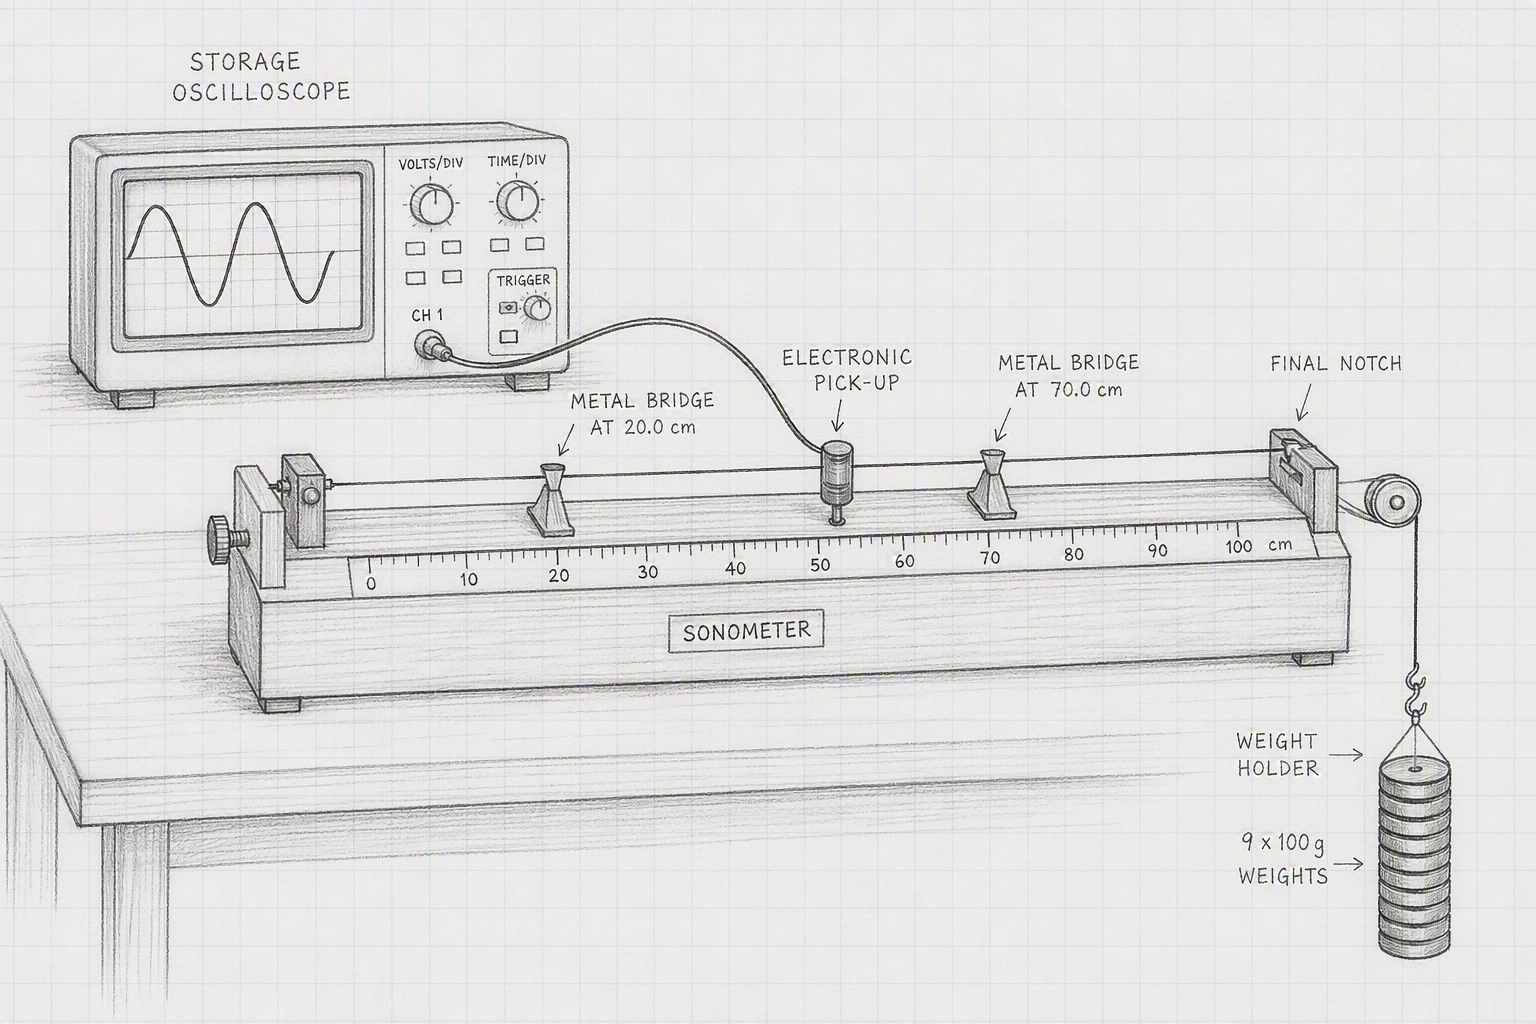
\includegraphics[width=10cm,height=5cm]{images/sonometer.png}

The apparatus will be set-up something like the sketch on the left.
Pluck te guitar wire in the centre and watch the trace on the
oscilloscope screen. When the trace settles down to a nice sinusoidal
shape after a second or so, press the pause button on the scope. The
frequency will be displayed on the scope screen. Record this, move the
weights to a different notch, and repeat the procedure.

\begin{itemize}
\item
  Record and note down the distance between the bridges on the
  sonometer. Measure to three decimal places in metres. This is \(L\).
  make sure this doesn't change over the experiment, i.e.~don't move the
  bridges.
\item
  Adjust the tension in the wire so that the lever arm is horizontal.
\item
  It is easiest to start at the fifth and furthest notch, i.e.~start
  from the bottom of the resuts table. It is easier to measure freuency
  for this setting.
\item
  When filling out your table, pay special attention to significant
  figures. The number of significant figures for \(f^2\) should be the
  same as for \(f\). Using scientific notation is a good idea here with
  powers of \(10^4\).
\end{itemize}

\newpage{}

\subsection{Analysis}\label{analysis-3}

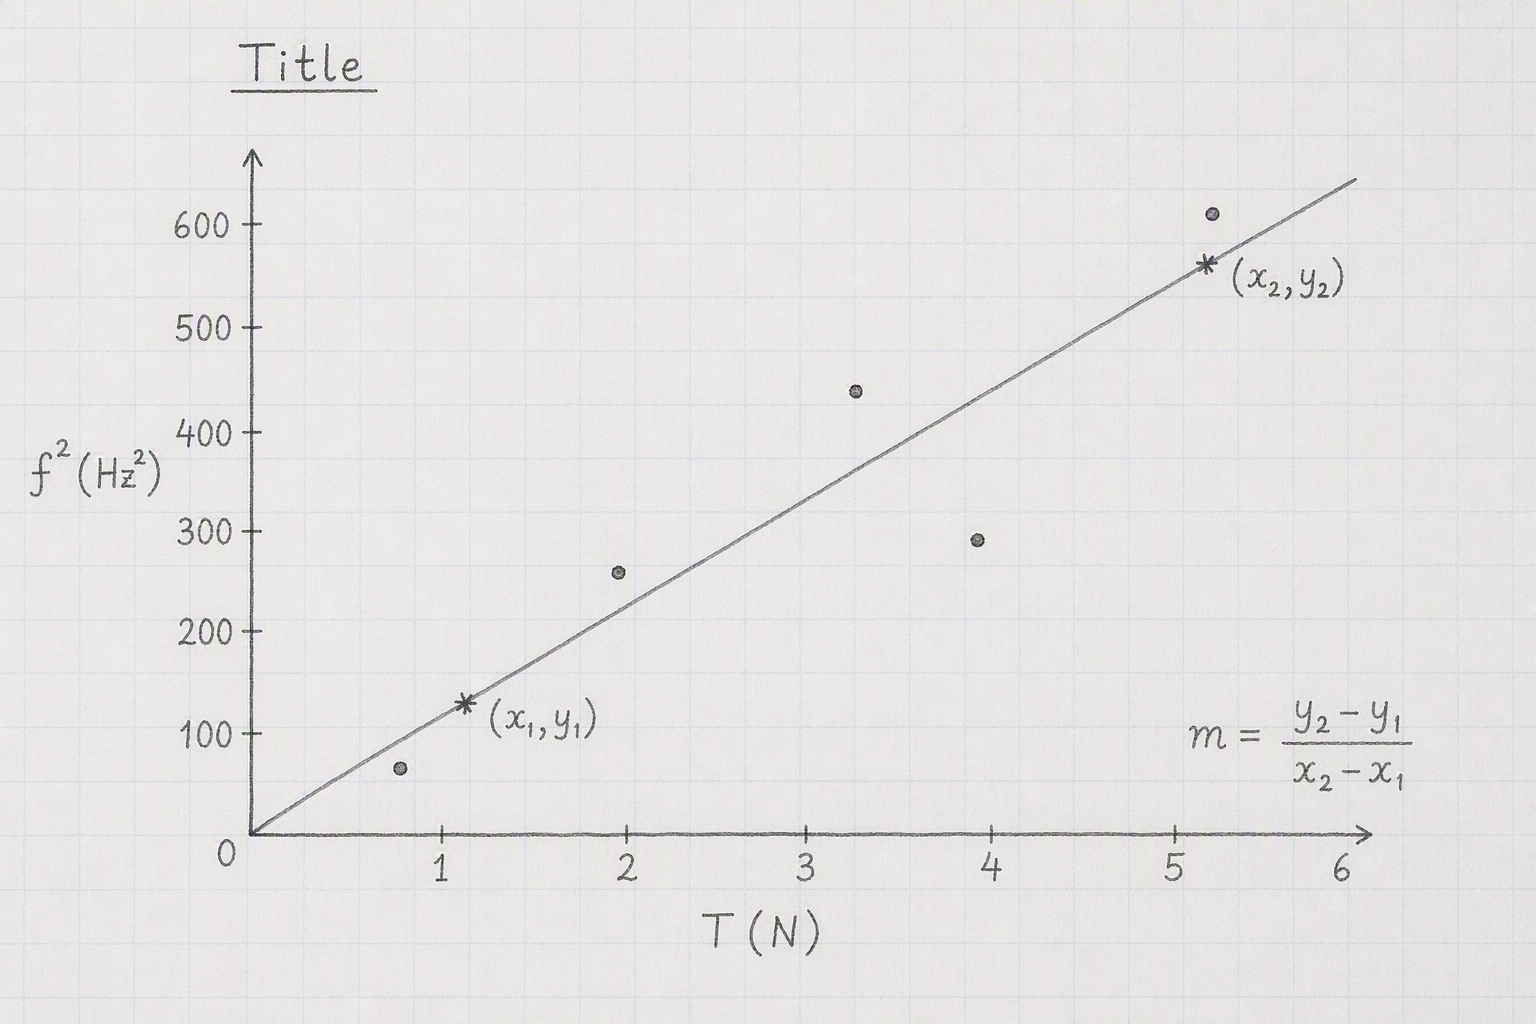
\includegraphics[width=10cm,height=6cm]{images/sonometer-graph.png}

Draw the graph as shown on the left here, with \(f^2(Hz^2)\) on the
y-axis and \(T(N)\) on the y axis. Draw a best fit line nested through
the points. Make sure the graph has a (long) descriptive title in the
form \emph{What's on y-axis vs What's on x axis and the context}.

Calculate the slope of the best fit line using the formula
\(slope \; = \; \frac{y_2-y_1}{x_2-x_1}\)

\subsection{\texorpdfstring{Calculation of the mass per unit length,
\(\mu\)}{Calculation of the mass per unit length, \textbackslash mu}}\label{calculation-of-the-mass-per-unit-length-mu}

The equation of relevance here is:
\(f \; = \; \frac{1}{2L} \sqrt{ \frac{T}{\mu}}\) where \(L\) is the
distant between the bridges that we measured.

Squaring both sides and rearranging we get
\(\mu \; = \; \frac{1}{4L^2 \times slope}\)

We're going to check on our \(\mu\) value by a separate set of
measurements. Detach the wire from the sonometer. Measure its entire
length, \(D\) in metres between the brass connectors at either end. Now
coil up the wire and measure its mass, \(m_{wire}\) on the scales.
Subtract 0.321g from the mass (this is the mass of the brass
connectors). Calculate a second value for \(\mu\) using:

\(\mu_{direct} \; = \; \frac{m_{wire} - 0.321}{D} \div 1000\) the factor
of 1000 is to convert grams to kg.

\subsection{Discussion}\label{discussion-3}

There are four parts to the discussion section:

Because we have two experimental values for \(\mu\), we'll combine our
results and textbook value in a table

\begin{itemize}
\tightlist
\item
  \textbf{\emph{the main results and manufacturer's value}}
\end{itemize}

\begin{table}
\fontsize{12.0pt}{14.0pt}\selectfont
\begin{tabular*}{\linewidth}{@{\extracolsep{\fill}}lr}
\toprule
Source & \mu(kgm^{-1}) \\ 
\midrule\addlinespace[2.5pt]
Sonometer &  \\ 
Direct &  \\ 
Manufacturer & 20.0 \\ 
\bottomrule
\end{tabular*}
\end{table}

\begin{itemize}
\item
  \textbf{\emph{inaccuracies}} - your values for \(\mu\) won't be
  exactly the same, nor will your graph be a perfect straight line. We
  need to try and account for these discrepancies. Pick one feature of
  the experiment and investigate whether it is an issue in the accuracy
  of your results. For example, how repeatable are the measurements of
  frequency from the oscilloscope, you could repeat several times for
  one value of T and see how consistent they are. You'll need to examine
  the results you have already as well as gathering additional evidence
  by taking further measurements. Your idea might well be a key issue in
  the quality of the results we obtain, or it might not be and you are
  thus ruling it out. Both are valid outcomes of this error analysis.
\item
  \textbf{\emph{improvements}} - based on the inaccuracy section above,
  can you suggest a way in which we could make our experiment better?
\end{itemize}

\subsection{Apparatus}\label{apparatus-3}

Sonometer with 0.17 gauge wire mounted (make sure to check the gauge,
should give diameter of mm). Two bridges set roughly 0.7m apart under
the wire. detector (not driver) coil connected to channel A of storage
oscilloscope. Scope set to \emph{measure} and \emph{frequency} on
\emph{Channel A}. Weight holder with total of 1kg. Check that frequency
measured from fifth notch is about 250Hz.

\bookmarksetup{startatroot}

\chapter{Focal Lenght of a Convex
Lens}\label{focal-lenght-of-a-convex-lens}

From the cornea in your eye to the camera of your phone, a lens is a
critical component of most optical systems. And for a lens, its focal
length is key parameter dictating its performance. In today's experiment
we will measure thefocal length of a convex (converging, thicker in the
center than at the edges) lens.

Take down the following in to your laboratory copy.

\subsection{\texorpdfstring{{Title: Focal Length of a Convex
Lens}}{Title: Focal Length of a Convex Lens}}\label{title-focal-length-of-a-convex-lens}

\subsection{\texorpdfstring{{Name:}}{Name:}}\label{name-4}

\subsection{\texorpdfstring{{Date:}}{Date:}}\label{date-5}

\subsection{\texorpdfstring{{Partner:}}{Partner:}}\label{partner-5}

\subsection{\texorpdfstring{{Data:}}{Data:}}\label{data-5}

\begin{table}
\fontsize{13.0pt}{15.0pt}\selectfont
\begin{tabular*}{0.85\linewidth}{@{\extracolsep{\fill}}>{\centering\arraybackslash}p{\dimexpr 90.00pt -2\tabcolsep-1.5\arrayrulewidth}>{\centering\arraybackslash}p{\dimexpr 90.00pt -2\tabcolsep-1.5\arrayrulewidth}>{\centering\arraybackslash}p{\dimexpr 90.00pt -2\tabcolsep-1.5\arrayrulewidth}>{\centering\arraybackslash}p{\dimexpr 90.00pt -2\tabcolsep-1.5\arrayrulewidth}}
\toprule
Object Distance, u, (cm) & Image Distance, v, (cm) & 1/u \((cm^{-1})\) & 1/v \((cm^{-1})\) \\ 
\midrule\addlinespace[2.5pt]
27.0 &  & 0.0370 &  \\ 
29.0 &  & 0.0345 &  \\ 
32.0 &  & 0.0312 &  \\ 
35.0 &  & 0.0286 &  \\ 
38.0 &  & 0.0263 &  \\ 
43.0 &  & 0.0233 &  \\ 
48.0 &  & 0.0208 &  \\ 
56.0 &  & 0.0179 &  \\ 
66.0 &  & 0.0152 &  \\ 
80.0 &  & 0.0125 &  \\ 
\bottomrule
\end{tabular*}
\end{table}

\subsection{Experimental Set-Up}\label{experimental-set-up-4}

\pandocbounded{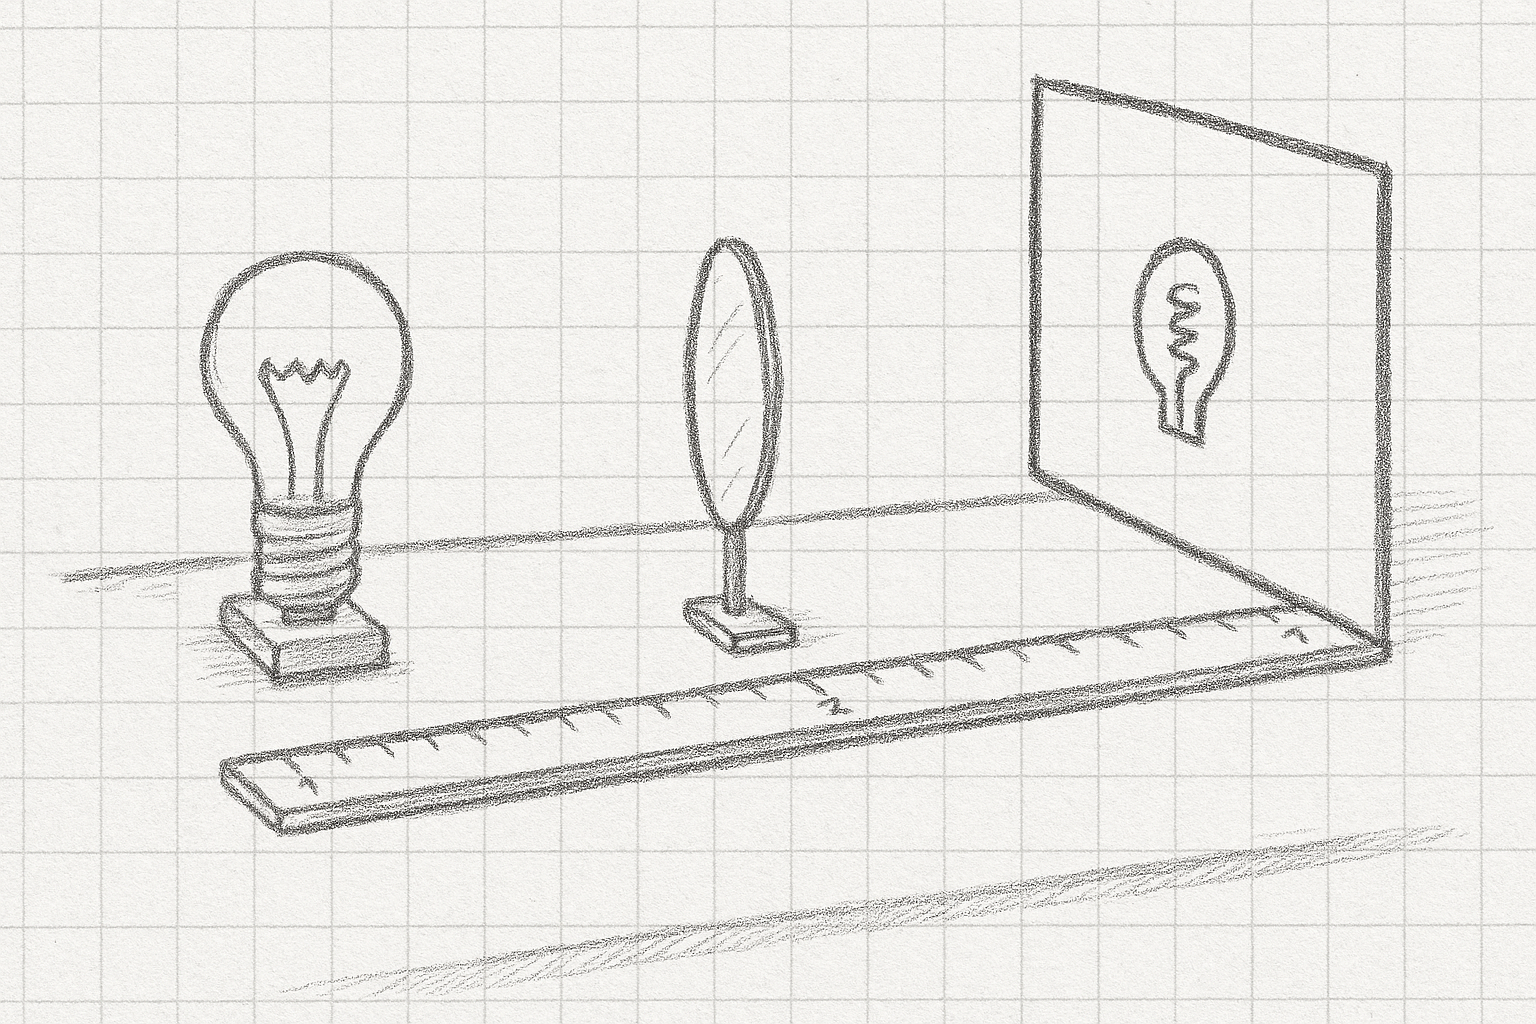
\includegraphics[keepaspectratio]{images/lens-setup.png}}

The apparatus will be set-up something like the sketch on the left. This
is the first point; the lens is quite close to the light source, the
screen is at the far end of the bench, and the spring-like image of the
bulb filament is quite large on the screen.

Set the distance between the center of the light source (not the front
edge) and the very centre of the lens to be 27.0cm and move the screen
until the light bulb filament in sharp focus. Measure the distance
between the centre of the lens and the screen. This is \(v\), the image
distance. Now move the lens back to 27.0 cm, move the screen in to get a
sharp focus, and record the new value for \(v\). Repeat for all the
values for \(u\) given in the table above.

\newpage{}

\begin{itemize}
\item
  \(u\) is measured from the middle of the light assembly, not the front
  edge
\item
  You get the sharpest focus images when you keep good geometry; the
  lens and screen being perpendicular to the light beam
\item
  initially the screen will move in towards the light source, but after
  about \(u\) = 43.0 cm is starts to move back again. The final point
  will have the lens and screen quite close together at the far end of
  the bench from the light and the image will be very small.
\item
  When filling out your table, pay special attention to significant
  figures. The number of significant figures for \(\frac{1}{v}\) should
  be the same as for \(v\).
\end{itemize}

\subsection{Analysis}\label{analysis-4}

\pandocbounded{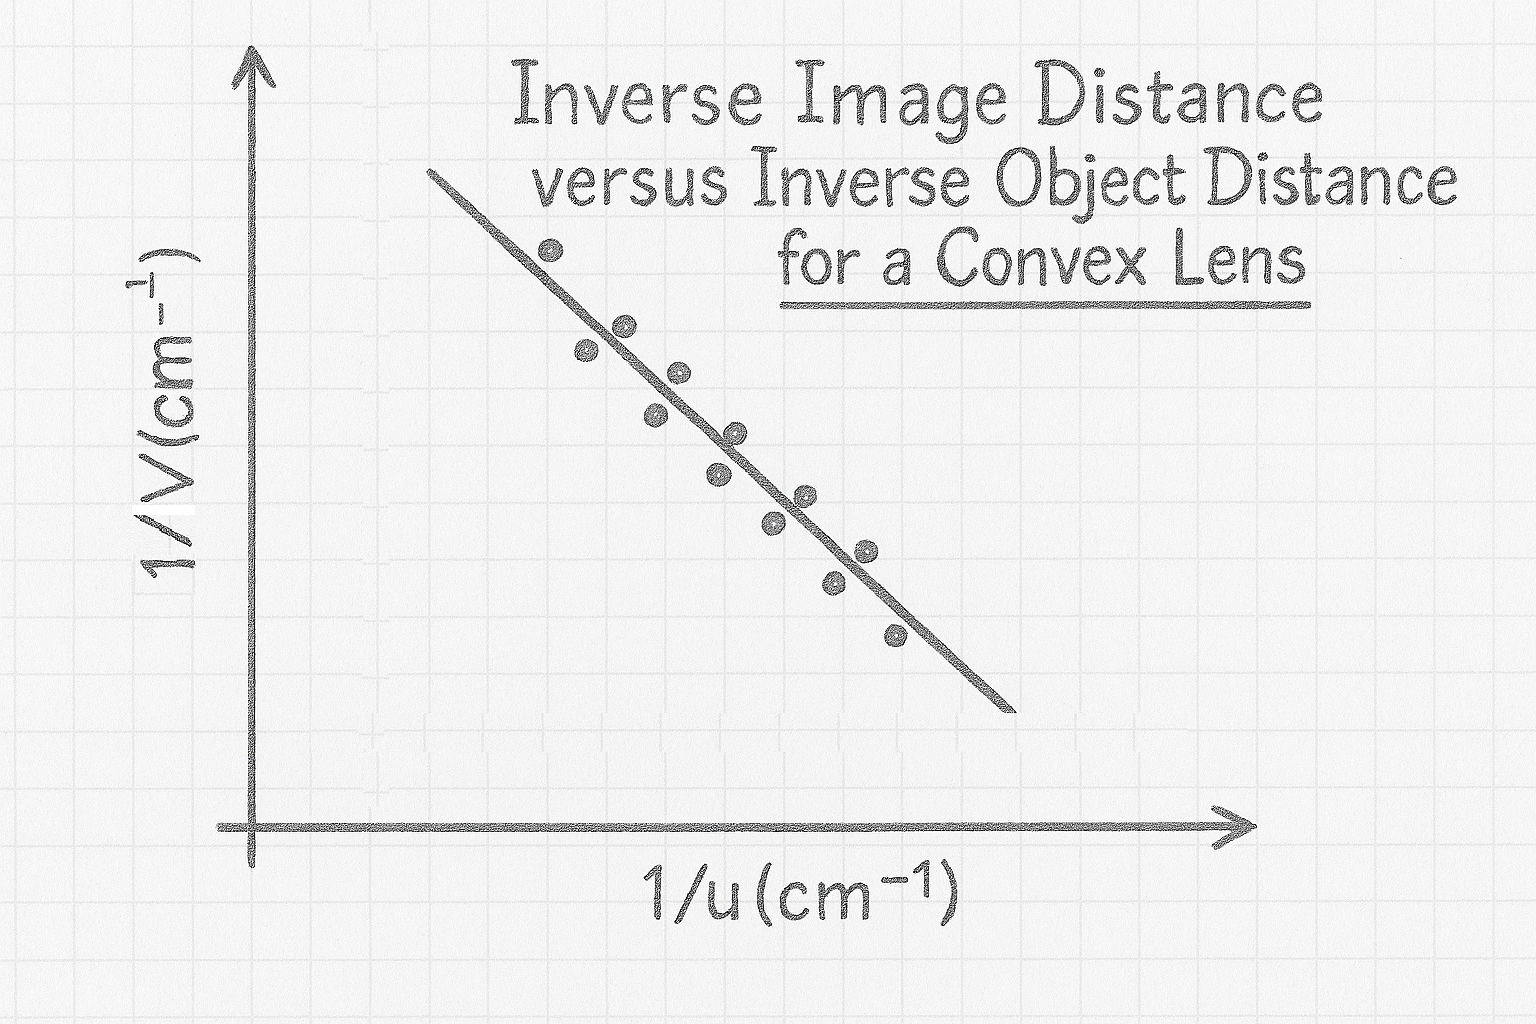
\includegraphics[keepaspectratio]{images/lens-graph.png}}

Draw the graph as shown on the left here, with \(\frac{1}{v}\) on the
y-axis and \(\frac{1}{u}\) on the x axis. Make sure both axes extend at
least as far as \(0.06 \: cm ^{-1}\), so for a standard
\(9 \; \times \; 13\) graph paper, use 0.01 per division on the x axis
and 0.005 per division on the y axis. Draw a best fit line nested
through the points. Make sure the graph has a (long) descriptive title
in the form \emph{What's on y-axis vs What's on x axis and the context}.

Calculate the slope of the best fit line using the formula
\(slope \; = \; \frac{y_2-y_1}{x_2-x_1}\)

According to theory (see below), this line should have a slope close to
-1. Note that, because it's a negative slope, the line angles downwards.

\subsection{Calculation of the Focal Length,
f(cm)}\label{calculation-of-the-focal-length-fcm}

The equation governing the focal length of a lens is:

\(\frac{1}{f} \; = \; \frac{1}{u} \; + \; \frac{1}{v}\)

\(\implies \frac{1}{v} \; = \; -\frac{1}{u} \; + \; \frac{1}{f}\) so
when \(\frac{1}{u}\) is zero, \(\frac{1}{v} \; = \; \frac{1}{f}\).

Take the point where the line cuts the y-axis, take the inverse of this
value, and this will be a figure for f.

\subsection{f from Direct Measurement}\label{f-from-direct-measurement}

Take the lens out to the lobby outside the lab and under one of the
ceiling lights. Hold the lens about 20 cm above the floor and get the
ceiling light in focus. Because the light source is so high above, then
\(u\) is very large and \(\frac{1}{u}\) is close to zero, then
\(\frac{1}{f} \; = \; \frac{1}{v}\) and the focal lenght will be well
approximated by the distance between the lens and the image on the
floor. Measure this to get a second estimate for f.

\subsection{f from no-parallax}\label{f-from-no-parallax}

\pandocbounded{\includegraphics[keepaspectratio]{images/no-parallax.png}}

Set up the apparatus as shown, with the object pin about 10cm behind the
lens and the retort stand and pencil about 20cm further back. Observe
the object pin through the lens and the pencil directly over the top rim
of the lens. Move the retort stand until the pencil sits directly over
the image of the object pin and the two stay in sync when you move your
head from side to side. Measure the distance from pin to lens, \(u\),
and the distance from pencil to lens, \(-v\). Put the values in to the
equation \(\frac{1}{f} \; = \; \frac{1}{u} \; + \; \frac{1}{v}\) to
calculate a value for f.

\newpage{}

\subsection{Discussion}\label{discussion-4}

There are four parts to the discussion section. Because we have three
experimental values for f, we'll combine our results and textbook value
in a table

\begin{itemize}
\tightlist
\item
  \textbf{\emph{the main results and manufacturer's value}}
\end{itemize}

\begin{table}
\fontsize{12.0pt}{14.0pt}\selectfont
\begin{tabular*}{\linewidth}{@{\extracolsep{\fill}}lr}
\toprule
Source & f (cm) \\ 
\midrule\addlinespace[2.5pt]
Graph &  \\ 
Lobby &  \\ 
No-Parallax &  \\ 
Manufacturer & 20.0 \\ 
\bottomrule
\end{tabular*}
\end{table}

\begin{itemize}
\item
  \textbf{\emph{supplementary main result}} - repeat your value for the
  slope of the graph and compare to the textbook value of -1.
\item
  \textbf{\emph{inaccuracies}} - your values for \(f\) won't be exactly
  the same as the manufacturers, nor will your graph be a perfect
  straight line with a slope of -1. We need to try and account for these
  discrepancies. Pick one feature of the experiment and investigate
  whether it is an issue in the accuracy of your results. You'll need to
  examine the results you have already as well as gathering additional
  evidence by taking further measurements. Your idea might well be a key
  issue in the quality of the results we obtain, or it might not be and
  you are thus ruling it out. Both are valid outcomes of this error
  analysis.
\item
  \textbf{\emph{improvements}} - based on the inaccuracy section above,
  can you suggest a way in which we could make our experiment better?
\end{itemize}

\subsection{Apparatus}\label{apparatus-4}

Light source, 20cm lens, screen, two metre sticks, retort stand, finder
pin, object pin.

\bookmarksetup{startatroot}

\chapter*{References}\label{references}
\addcontentsline{toc}{chapter}{References}

\markboth{References}{References}

\phantomsection\label{refs}
\begin{CSLReferences}{0}{1}
\end{CSLReferences}




\end{document}
